\documentclass{article}

\usepackage[preprint]{neurips_2025}
\usepackage[utf8]{inputenc}
\usepackage[T1]{fontenc}
\usepackage{hyperref}
\usepackage{url}
\usepackage{booktabs}
\usepackage{graphicx}
\usepackage{amsmath}
\usepackage{microtype}

\title{Balanced Hybrid KVPress Compression for Training-Free Pythia-70M Inference}

\author{%
  Group Project Team\\
  Shanghai Jiao Tong University\\
  \texttt{https://github.com/SJTU-huaxing/llm-hw-team.git}
}

\begin{document}

\maketitle

\begin{abstract}
KV cache compression reduces autoregressive inference memory, but aggressive pruning often trades quality for speed. We study this tradeoff on EleutherAI/Pythia-70M with NVIDIA KVPress, no training, and fp32 eager attention. Beyond Dense, StreamingLLM, SnapKV, PyramidKV, ExpectedAttention, ObservedAttention, and TOVA baselines, we implement two KVPress-compatible hybrid presses. The selected method, Hybrid Expected-Observed, combines expected future attention, observed heavy-hitter attention, and value norm scores while protecting sink and recent tokens. At a 132-token target cache for a 512-token context, it lies on the Pareto frontier and has the best equal-rank balance over average perplexity, TPOT, and decode-attention FLOPs, while ExpectedAttention remains the strongest quality baseline. We report the negative result that adding a soft pyramid budget did not improve the simpler hybrid, and provide code, results, plots, and a reproducible Conda environment.
\end{abstract}

\section{Introduction}

The KV cache stores one key and value vector per layer and token, so long-context decoding stresses GPU memory and attention bandwidth. The assignment asks us to combine ideas from four levels: attention mechanisms, per-layer KV eviction, inter-layer cache allocation, and macro inference architecture. We keep the model fixed, use no training, and use KVPress~\citep{kvpress} to hook Transformers during prefill.

Pythia-70M~\citep{biderman2023pythia} uses GPT-NeoX attention modules and partial RoPE, while several KVPress utilities assume LLaMA-like module names and full-dimensional RoPE. Our adapter only supplies these structural aliases and the partial-RoPE correction needed for ExpectedAttention. All compression decisions are implemented as KVPress-style presses that gather existing KV tensors along the sequence dimension.

\section{Method}

Table~\ref{tab:layers} summarizes how the implementation covers the assignment layers. Official baselines include attention sink retention~\citep{xiao2023streamingllm}, observed attention from SnapKV/PyramidKV~\citep{li2024snapkv,cai2024pyramidkv}, H2O-style heavy-hitter scoring~\citep{zhang2023h2o}, and TOVA~\citep{tova2024}.

\begin{table}[h]
\centering
\small
\caption{Mapping from acceleration layers to implemented components.}
\label{tab:layers}
\begin{tabular}{ll}
\toprule
Layer & Components \\
\midrule
Attention mechanism & ExpectedAttention, ObservedAttention/TOVA, value norm \\
Per-layer compression & StreamingLLM, SnapKV, PyramidKV, observed/top-$k$ scorers \\
Inter-layer compression & Pyramid budgets, lazy gate, soft hybrid budget ablation \\
Macro architecture & KVPress pipeline, prefill-once compression, unified timing \\
\bottomrule
\end{tabular}
\end{table}

Hybrid Expected-Observed uses
\[
s = 0.55\,\hat{s}_{\mathrm{expected}} + 0.30\,\hat{s}_{\mathrm{observed}} + 0.15\,\hat{s}_{\mathrm{vnorm}},
\]
where each score is min-max normalized per batch and head. Sink tokens and a 32-token recent window receive a protection boost before top-$k$ selection. Hybrid Soft Pyramid uses the same score but allocates a mild layer budget from low to high layers with factors from 1.25 to 0.75 and a floor of sink plus recent tokens. This tests whether layer non-uniformity helps once the token scorer is already hybrid.

\section{Experiments}

We evaluate `EleutherAI/pythia-70m' on WikiText-2 test~\citep{merity2017wikitext} and one PG-19 test stream sample~\citep{rae2019compressive}. For PPL, a 512-token context is prefetched and compressed before scoring the next 128 continuation tokens. For generation, a 512-token PG-19 prompt generates 32 tokens. The decode attention FLOPs proxy is $\sum_{\ell,t}4HDL_{\ell,t}$. Reported runs use an NVIDIA GeForce RTX 5060 Laptop GPU.

We first screen new baselines and hybrids on 256-token contexts and target cache sizes 96, 128, and 192. The strongest new official baselines are ObservedAttention and TOVA, so the final table keeps them alongside the original methods. The balanced selection rule filters methods with kept fraction above 0.5 and ranks the remaining methods by average PPL, TPOT, and FLOPs ratio with equal weight.

\begin{table}[h]
\centering
\small
\caption{Target cache 132. PPL is averaged over WikiText-2 and PG-19; generation is on PG-19.}
\label{tab:main}
\begin{tabular}{lrrrr}
\toprule
Policy & Avg PPL & Kept & TPOT & FLOPs \\
\midrule
Dense & 21.344 & 1.000 & 0.00579 & 1.000 \\
ExpectedAttention & 26.326 & 0.258 & 0.00580 & 0.281 \\
Expected+Pyramid & 35.066 & 0.259 & 0.00572 & 0.282 \\
Layer-adaptive Expected+Pyramid & 37.279 & 0.259 & 0.00577 & 0.282 \\
Hybrid Expected-Observed & 37.870 & 0.258 & 0.00575 & 0.281 \\
Hybrid Soft Pyramid & 38.884 & 0.258 & 0.00576 & 0.281 \\
ObservedAttention & 40.107 & 0.258 & 0.00572 & 0.281 \\
StreamingLLM & 46.148 & 0.258 & 0.00587 & 0.281 \\
TOVA & 53.386 & 0.258 & 0.00588 & 0.281 \\
\bottomrule
\end{tabular}
\end{table}

\begin{table}[h]
\centering
\small
\caption{Balanced selections across target cache sizes.}
\label{tab:budget}
\begin{tabular}{lrrrr}
\toprule
Target & Selected policy & Avg PPL & TPOT & FLOPs \\
\midrule
132 & Hybrid Expected-Observed & 37.870 & 0.00575 & 0.281 \\
192 & ExpectedAttention & 22.407 & 0.00599 & 0.395 \\
256 & Hybrid Expected-Observed & 26.329 & 0.00574 & 0.516 \\
\bottomrule
\end{tabular}
\end{table}

\begin{figure}[h]
\centering
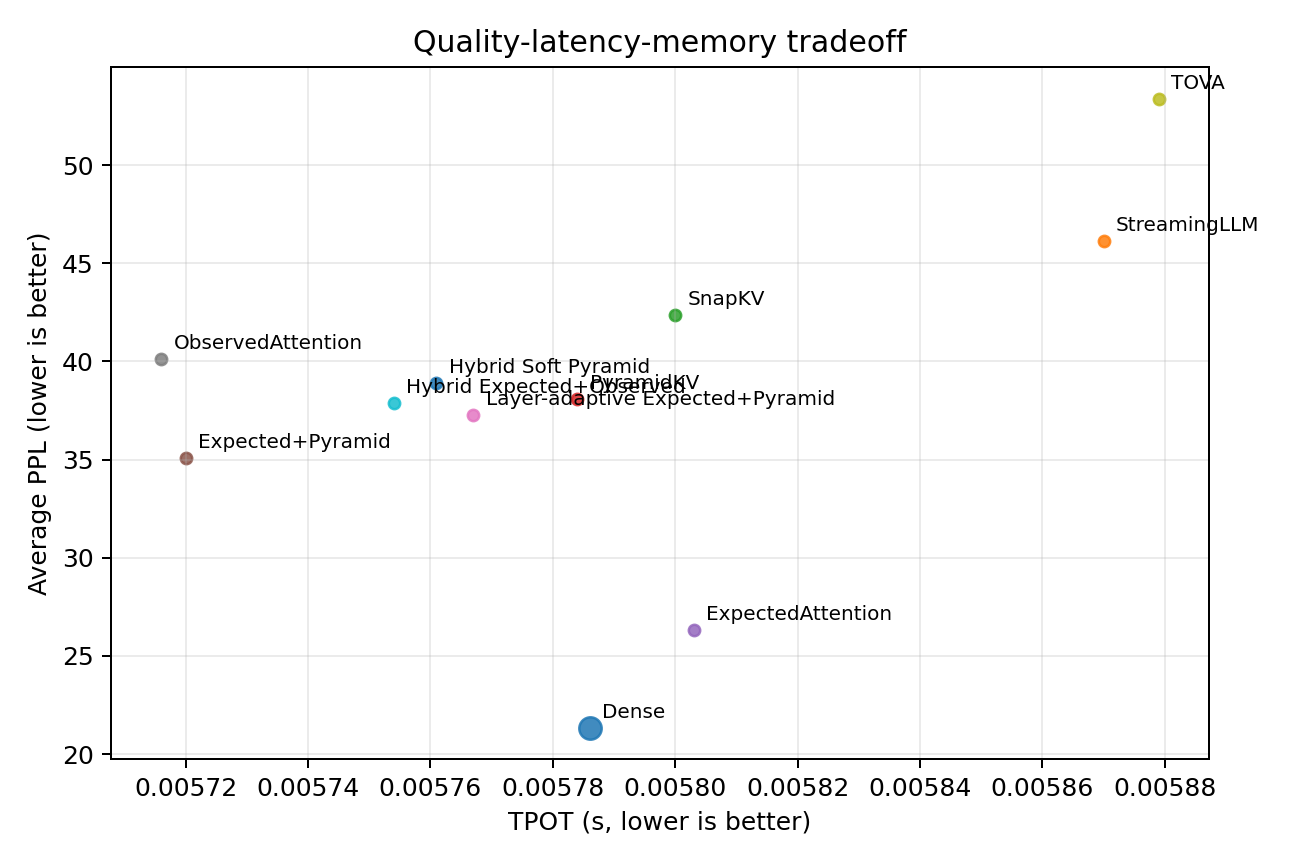
\includegraphics[width=0.70\linewidth]{../results/quality_latency_tradeoff.png}
\caption{Average PPL versus TPOT at target cache 132.}
\label{fig:tradeoff}
\end{figure}

\section{Analysis and Limitations}

The main result is not that the hybrid scorer always minimizes PPL. ExpectedAttention is clearly the quality anchor, especially on WikiText-2. The hybrid is selected by the assignment's balanced rank because its TPOT is close to the fastest policies while preserving a moderate quality level under aggressive compression. Hybrid Soft Pyramid is a useful negative ablation: adding layer non-uniformity to the hybrid score does not dominate the simpler uniform-budget hybrid.

The evaluation is intentionally small and reproducible: one model, no training, two datasets, fixed seeds, and one GPU. Timing differences are small at Pythia-70M scale, so the paper reports exact CSVs rather than over-claiming hardware speedups. We do not implement MQA/GQA/MLA or YOCO-style cross-layer sharing because those require architecture or weight changes outside the no-training setting. KVPress SimLayerKV is excluded because its full-RoPE assumption is incompatible with GPT-NeoX partial RoPE without further changes.

\section{Team Contributions}

Replace these placeholders with final member names and IDs before submission. Member A: method design and implementation (40\%). Member B: experiments and analysis (35\%). Member C: paper writing and reproducibility (25\%).

\bibliographystyle{plainnat}
\bibliography{references}

\end{document}
